\section{Summary}

A selection designed to be uniformly efficient in all regions of the dark boson's mass-lifetime
parameter space has been presented with a view to embark in a search for a new dark boson.
A frequentist method designed to search for an excess in any arbitrary mass spectrum has also been
presented and used in the case of the dimuon mass spectrum from \btokstrmumu.

This strategy has extracted a $p$-value of a particle considering test masses which do not go all
the way to the boundaries of various vetoes in the invariant dimuon mass spectrum.
It is determined that the maximum deviation of the selected candidates from the null hypothesis of
zero signal has a global significance of $0.48\stdev$ at $m_t = 4285.0\mev$.
This is consistent with no new particle in the \mumu distribution.
The full analysis will get much closer to these edges and probe the interesting $m_{\mumu}=214\mev$
region.
The next step in the analysis is to set limits and present them in a model independent way.
Of course, they can be translated to specific models for interpretation.

%Figure~\ref{fig:db:excl} shows projected exclusion regions from this analysis.
%Figure~\ref{fig:db:excl:inf} shows projected exclusion regions for the inflaton
%model~\cite{Bezrukov:2014nza}, and axion model~\cite{Freytsis:2009ct}.

Figure~\ref{fig:db:excl:infl} shows that the projected
sensitivity of this analysis, for an inflaton model~\cite{Bezrukov:2014nza},
should be sufficient to rule out the range
$250<\mass{\db}<450\mev$ and come within an oder of magnitude of the allowed region up to
$1000\mev$.
There is a region excluded by theory, where the model does not satisfy known cosmological
constraints.
Assumptions made in making this, are that the lifetime of the inflaton is in the range
$1<\lifetime{db}<1000\ps$, that  $\BF(\btokstrdb)\simeq10^{-6}$, and that $\BF(\dbtomumu)$
is the same for a Higgs boson with the mass of an inflaton.

\begin{figure}
  \begin{center}
    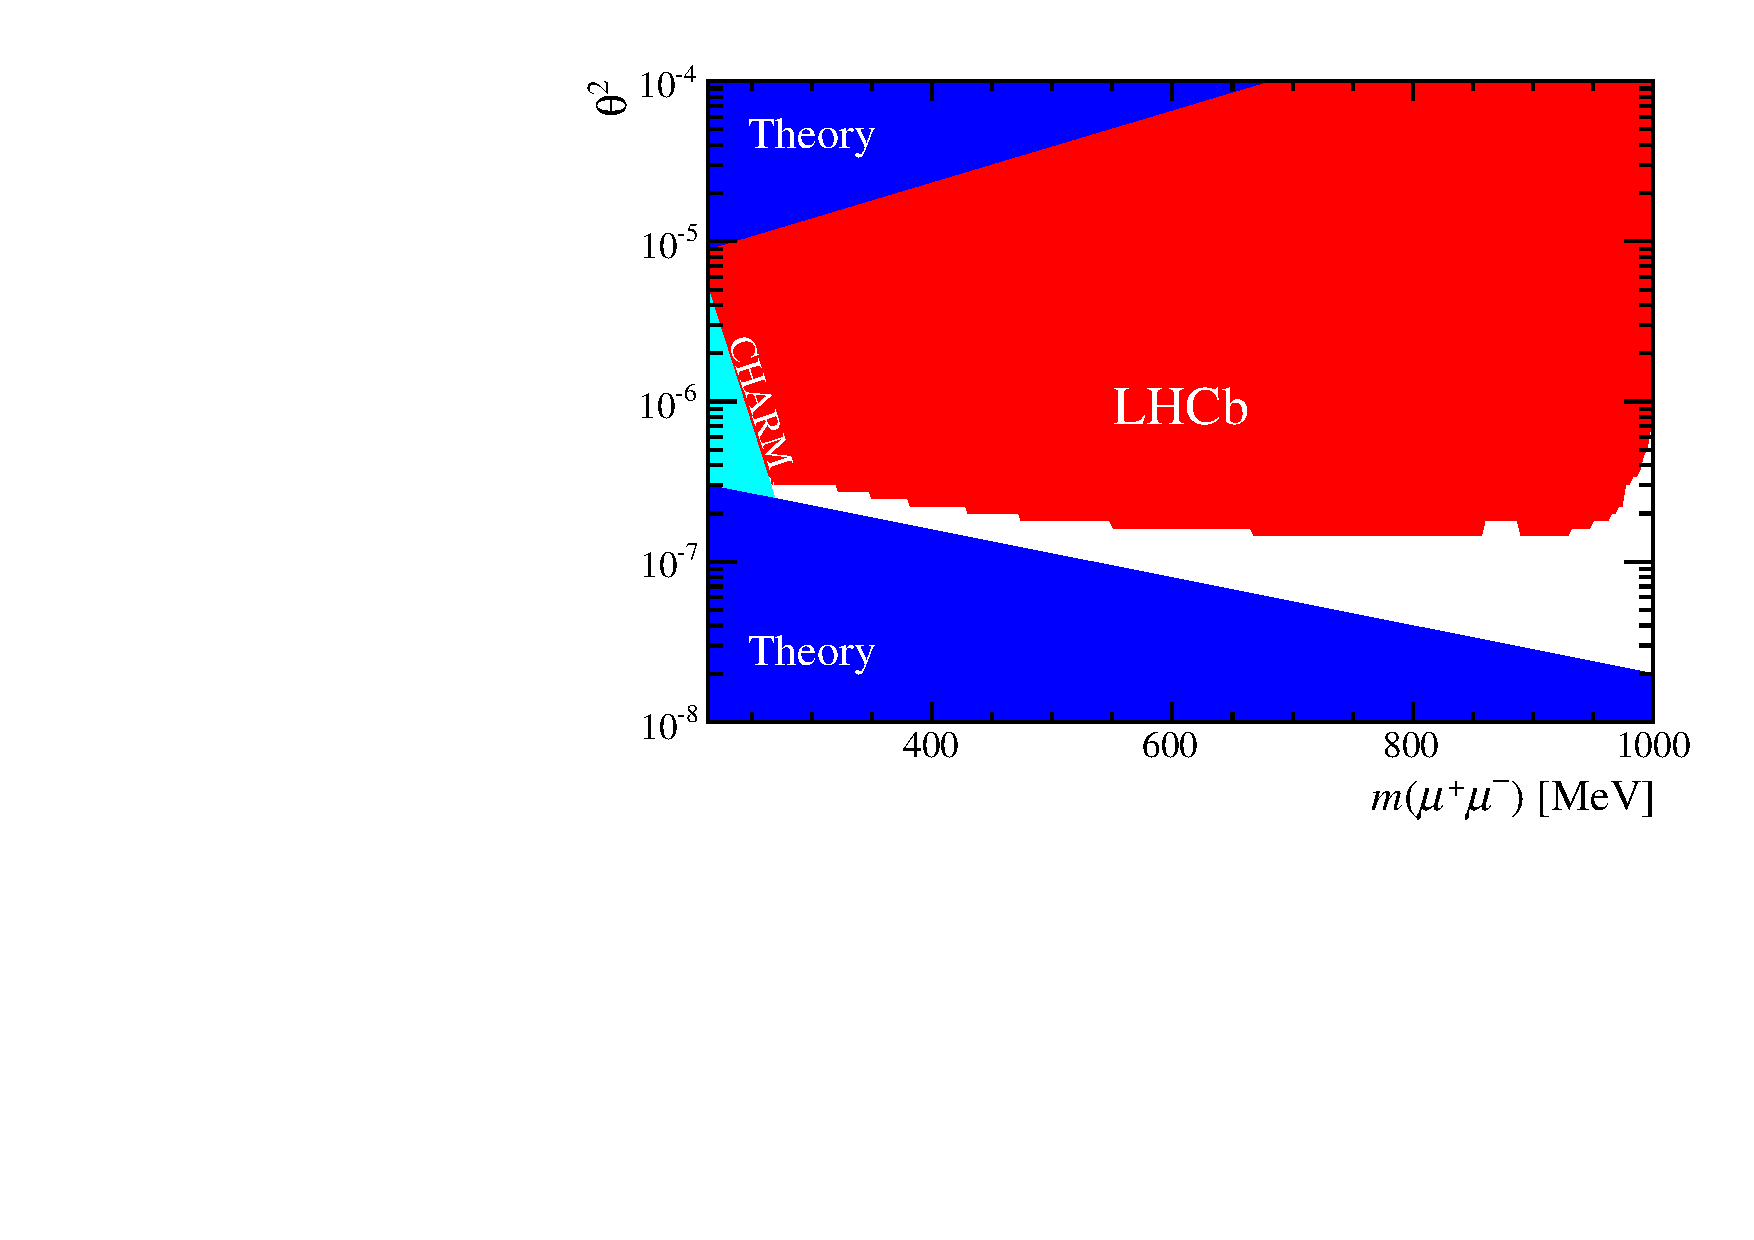
\includegraphics[width=0.6\textwidth]{kstmm_infl_excl}
    \caption[Projected sensitivity in an inflaton search]
    {
      Projected exclusions for an inflaton model from Ref.~\protect\cite{Bezrukov:2014nza}, in the
      mass range $1<\mass{\db}<1000\mev$.
      The region below the red line is excluded by theory, since the model fails cosmological
      constraints in this region.
      In this mass range, it is expected that this analysis will exclude all but a small area of
      parameter space for this model.
    }
    \label{fig:db:excl:infl}
  \end{center}
\end{figure}

%Figure~\ref{fig:db:excl:ax} shows that the regions of excluded parameter space for a model with an
%%axion $a$, as described in Ref.~\cite{Freytsis:2009ct}.
%It is observed that the excluded region is much smaller as $\mass{a}\geq2m_\tau$, because above
%this threshold $\BF(\decay{a}{\tau^+\tau^-})$ dominates.
%There is an additional complication coming from the unknown branching fraction of the axion to
%hadronic final states, \Fig{fig:db:excl:ax} shows the excluded range for
%$\BF(\decay{a}{\mathrm{hadrons}})=0$ and 0.99.
%The difference between these values of $\BF(\decay{a}{\mathrm{hadrons}})$ results in only a factor
%of \approx$2$, this is because as $\BF(\decay{a}{\mathrm{hadrons}})$ increases, \lifetime{a} must
%decrease because $\Gamma(\decay{a}{\mathrm{leptons}})$ is fixed.
%
%\begin{figure}
  %\begin{center}
    %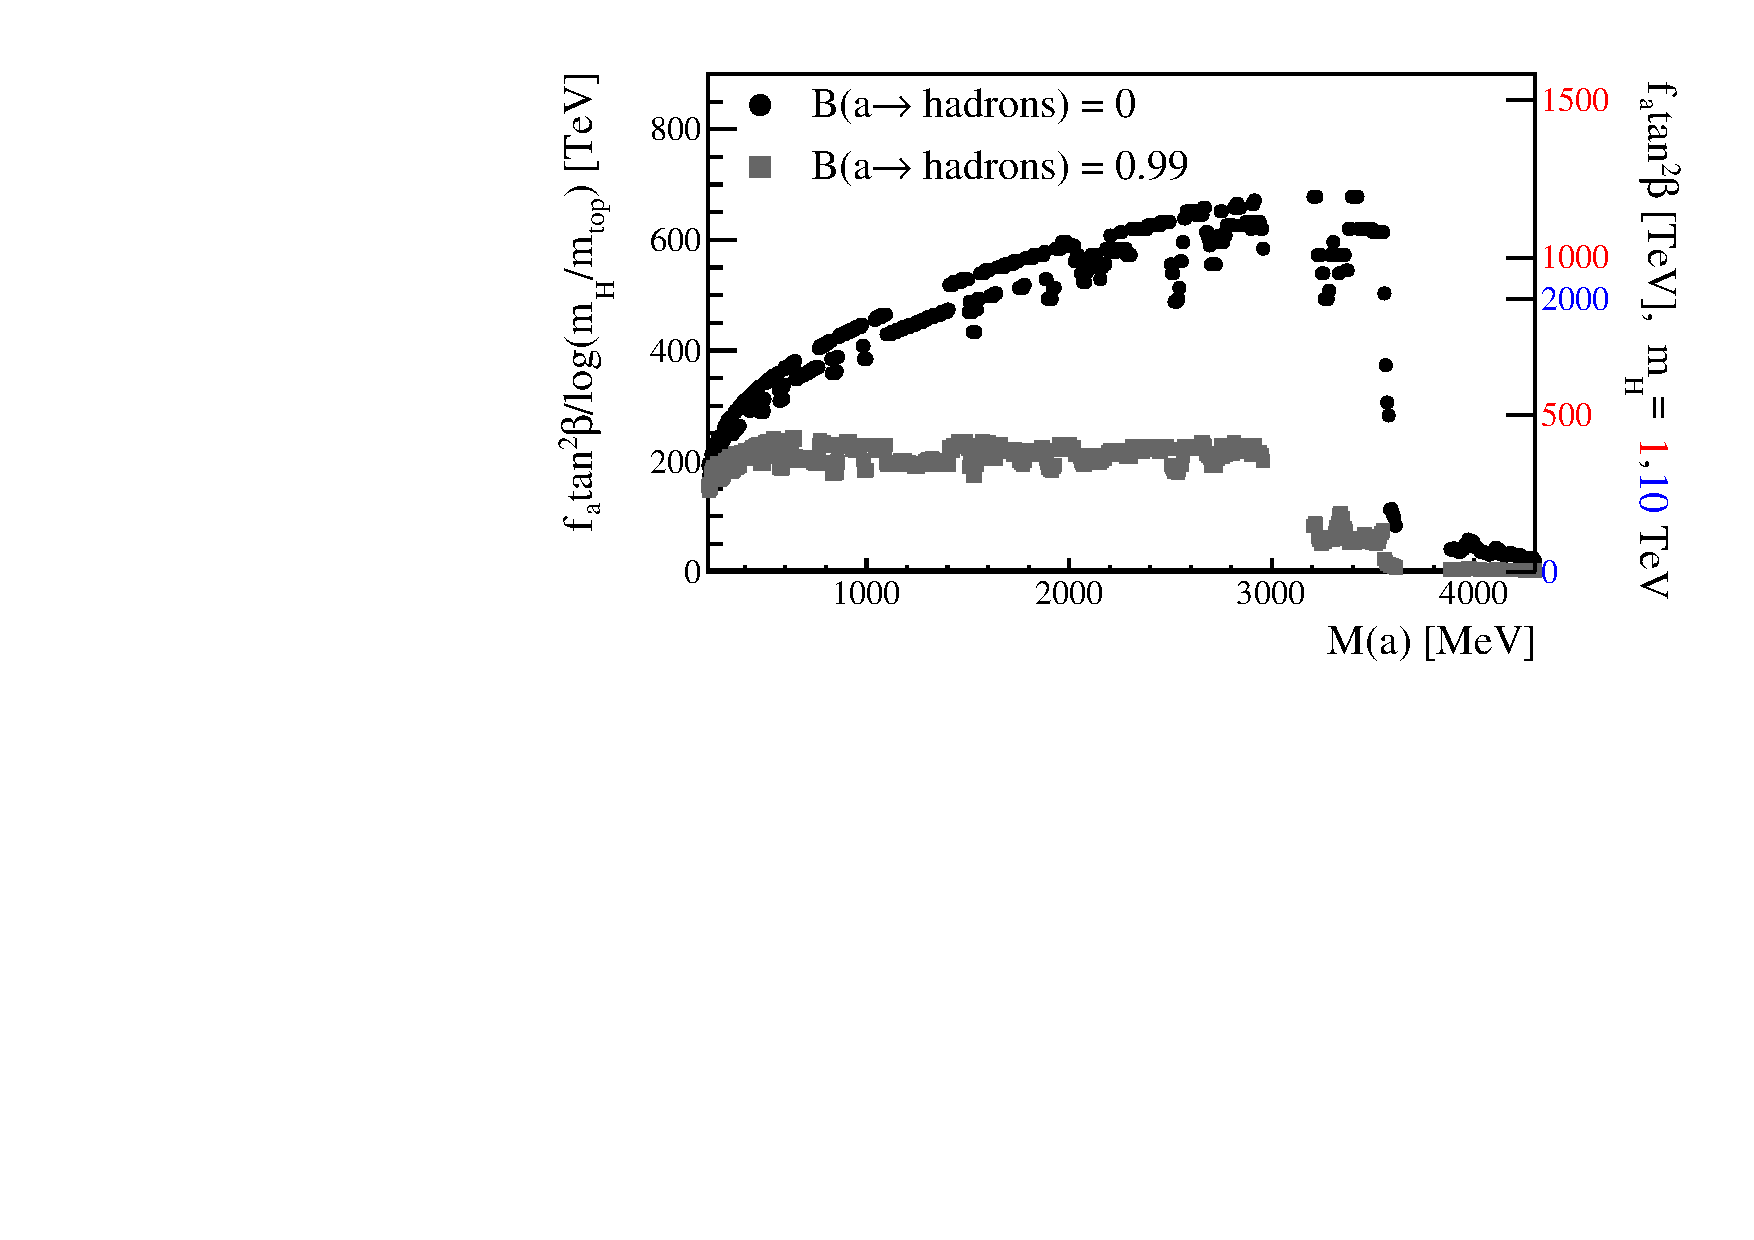
\includegraphics[width=0.48\textwidth]{kstmm_axion_excl}
    %\caption[Projected sensitivity in an axion search]
    %{
      %Projected exclusions for an axion model from Ref.~\protect\cite{Freytsis:2009ct}.
      %The region under the points is excluded, and two sets of points each depending on the
      %branching fraction of the $a$ to hadrons, which varies greatly in axion models but is usually
      %between 0 and 0.99 for all values of axion mass.
      %Limits shown are valid in the region $\tan\beta\gtrsim3$ and $m_H\gtrsim800\gev$, where
      %$\tan\beta$ is the ratio of \glspl{VEV} of the two Higgs bosons in a \gls{twoHDM}.
      %The right-hand colour axes show the explicit limits on $f_a\tan^2\beta$ for $m_H=1$ and
      %$10\tev$.
    %}
    %\label{fig:db:excl:ax}
  %\end{center}
%\end{figure}


%At the time of writing, this analysis is undergoing the review procedure and unblinding is ongoing.
%
%The plan is to unblind etc, and then fit if find $>3\sigma$ excess.
%
%Here, a fully frequentist method of searching for a dark boson with an unknown mass and lifetime
%has been presented.
%Specific peaking backgrounds are removed before the combinatorial background is suppressed by
%applying a \uBDT designed to yield a response which is uniform in signal efficiency in both the
%mass and lifetime dimensions.

%\begin{itemize}
  %\item New strategy
  %\item Excellent selectio
  %\item Excellent parmeterization
  %\item Sensitive
%\end{itemize}



